% SLIM-ARC: 学术报告 - 总结与未来展望
\section{总结与未来展望}

\subsection{工作总结}

本文提出了 SLIM-ARC，一个面向端侧 MoE 大模型推理的操作系统级协同优化框架。通过系统性分析和实验验证，我们做出了以下贡献：

\subsubsection{核心技术贡献}

\begin{enumerate}
    \item \textbf{发现并利用了 MADV\_RANDOM 对 MoE decode 的加速效应}：通过四组单点消融实验，精确定位了 \texttt{posix\_madvise(MADV\_RANDOM)} 是 decode 阶段加速的核心驱动因素。其作用机制是：关闭内核顺序预读后，仅被 MoE Router 激活的专家权重页面（10/512 = 2\%）通过 page fault 按需加载，其余 98\% 的未激活专家权重完全不占用物理内存。

    \item \textbf{识别并消除了 GGML\_CPU\_REPACK 的内存翻倍问题}：发现 llama.cpp CPU 后端的 Q4\_K $\to$ q4\_K\_8x8 重打包机制会导致匿名内存翻倍（45\,GB $\to$ 90\,GB），是 80B 模型在受限环境下 OOM 的根因。通过 \texttt{-DGGML\_CPU\_REPACK=OFF} 禁用该机制，使模型从 OOM 转变为可运行。

    \item \textbf{构建了完整的优化技术栈}：将 IQ4\_XS 模型量化、KV Cache Q4\_0 量化、层感知预取调度器、MoE Router 跨层专家预测、统一 I/O 调度器等优化技术有机集成，形成了从模型加载到运行时调度的完整优化链条。

    \item \textbf{实现了 80B 模型在端侧的流畅运行}：在 32\,GB 热缓存环境下，IQ4\_XS 量化的 Qwen3-Next-80B 达到了 \textbf{2.45\,tokens/s} 的 decode 速度（0.4 秒/token），实现了流畅的交互式推理。在 8\,GB 最受限环境下，达到了 0.76\,tokens/s，相比 baseline 提升 850\%（9.5 倍）。
\end{enumerate}

\subsubsection{实验验证}

通过三档 cgroup 环境（8/12/16\,GB）、三种模型（Qwen3-4B Dense、OLMoE-1B-7B MoE、Qwen3-Next-80B MoE）、四组单点消融、多种量化格式（Q4\_K\_M、IQ4\_XS、Q8\_0）的系统化实验，验证了：

\begin{itemize}
    \item MADV\_RANDOM 对大模型（>6\,GB）的 MoE decode 加速有效（+200\%$\sim$+850\%）
    \item 对小模型（<6\,GB），自适应跳过机制避免了不必要的开销
    \item KV Cache Q4\_0 量化带来 +14\% 的 decode 提升
    \item IQ4\_XS 相比 Q4\_K\_M 减少模型体积 5.4\,GB，热缓存速度提升 98\%
    \item prefetch\_scheduler 在当前场景下冗余，诚实评估了其贡献边界
\end{itemize}

\subsection{诚实评估与局限性}

\subsubsection{prefetch\_scheduler 的冗余}

四组消融实验明确表明，在 80B 模型 8\,GB/6\,GB 环境下，prefetch\_scheduler 没有独立贡献。原因是：在有 MADV\_RANDOM 时，内核的 page fault 机制已经足够按需加载，额外的 \texttt{madvise(WILLNEED)} 调用是冗余的；在无 MADV\_RANDOM 时，内核的默认 WILLNEED 策略已经全预读，prefetch 同样冗余。

这一发现的深层原因是：MoE 模型的 decode 访存模式虽然是稀疏的，但每层的激活专家权重仍然需要从 SSD 加载。在 NVMe 带宽（$\sim$3.5\,GB/s）远大于单层权重 I/O 需求的情况下，内核的 page fault 机制已足够高效，用户态预取调度的开销（madvise 系统调用 + 线程同步）反而抵消了其理论收益。

\subsubsection{数据波动问题}

80B 模型在受限环境下的性能数据存在显著波动（同一配置 tg8 从 0.28 到 1.03）。这源于 45\,GB 模型与 8--32\,GB 物理内存之间的巨大差距，导致每次推理的 page cache 命中率高度依赖系统状态。虽然通过冷启动（drop\_caches）和多次测量缓解了部分波动，但这一问题在大模型受限推理中是固有的。

\subsubsection{Phase 2b KV Cache 换页的未完成}

KV eviction manager 的接口已完整实现（register\_block、evict\_block、prefetch\_block、run\_eviction），但与推理流程的深度集成（hook KV cache 的 allocation/access 路径）尚未完成。当前仅在 \texttt{clear()} 方法中实现了 DONTNEED 页面释放。

\subsubsection{动态 MADV 切换的失效}

动态 MADV 切换（prefill $\to$ WILLNEED, decode $\to$ MADV\_RANDOM）在 llama-bench 的分离测试场景下表现不佳，因为 WILLNEED 预读的页面在切换到 MADV\_RANDOM 时会被丢弃。在真实推理（连续 prefill $\to$ decode 过渡）中可能有效，但需要进一步验证。

\subsection{未来展望}

\subsubsection{短期优化方向}

\begin{enumerate}
    \item \textbf{更激进的模型量化}：尝试 Q2\_K（$\sim$28\,GB）或 IQ2\_XXS（$\sim$22\,GB），进一步缩小模型体积以适应 8\,GB 环境。预计在 32\,GB 热缓存下可全量缓存，消除数据波动。

    \item \textbf{KV Cache 换页深度集成}：完成 \texttt{kv\_eviction\_manager} 与推理流程的集成，实现基于注意力分数的 KV Block 级别驱逐和预取，解决长上下文场景的内存瓶颈。

    \item \textbf{prefetch 价值场景探索}：在更长上下文（32K+）或更小内存（4\,GB）场景下重新评估 prefetch\_scheduler 的价值。当前测试的 context=1--32 token 下 KV 压力过小，可能不足以体现 prefetch 的协同效果。
\end{enumerate}

\subsubsection{中长期研究方向}

\begin{enumerate}
    \item \textbf{prefill/decode 动态 MADV 切换的优化}：设计更精细的切换策略，避免 WILLNEED 预读页面的浪费。例如，仅在 prefill 的第一个 ubatch 使用 WILLNEED，后续切换到 MADV\_RANDOM。

    \item \textbf{投机解码集成}：利用小模型（如 Qwen3-4B）作为 draft model，大模型（80B）作为 verifier，通过批量验证多个 token 来摊薄 I/O 成本。llama.cpp 已原生支持 \texttt{--spec-type ngram-simple}，但冷启动加载时间过长，需要优化。

    \item \textbf{Tile 级微流水线}：将权重张量切分为 Tile（对齐 L2/L3 cache 行），I/O 线程读 Tile-N 时计算线程处理 Tile-N-1。当前依赖内核 page cache 的隐式 Tile 机制，显式 Tile 级控制可能带来 20--40\% 的 cache 命中率提升。

    \item \textbf{统一调度器的协同验证}：完成 KV Cache 换页集成后，验证统一 I/O 调度器在权重预取 + KV 换页 + 专家预取三路竞争下的"协同 > 单点之和"效果。
\end{enumerate}

\subsection{结论}

SLIM-ARC 证明了一个关键 insight：\textbf{MoE 模型的专家稀疏性与操作系统虚拟内存机制的结合，是实现端侧大模型推理的有效路径}。通过 \texttt{madvise(MADV\_RANDOM)} 这一简单的内核接口调用，系统能够精确地只加载被激活的专家权重，将 45\,GB 模型的物理内存占用降至接近实际访问量（$\sim$2\,GB）。

这一发现对端侧 AI 部署具有实际意义：它表明，在不需要复杂用户态内存管理（如 FlexInfer 的 Direct I/O + 手动 buffer 管理）的情况下，仅通过操作系统虚拟内存的按需分页机制，就能实现大模型在受限环境下的运行。关键在于正确配置 madvise 策略以匹配 MoE 模型的稀疏访存模式。

最终，SLIM-ARC 使 Qwen3-Next-80B（45\,GB）在 8\,GB RAM 环境下从 OOM 变为可运行（0.76\,t/s），在 32\,GB 热缓存环境下达到流畅运行（2.45\,t/s），相比 baseline 实现了最高 850\%（9.5 倍）的性能提升。

\begin{figure}[H]
    \centering
    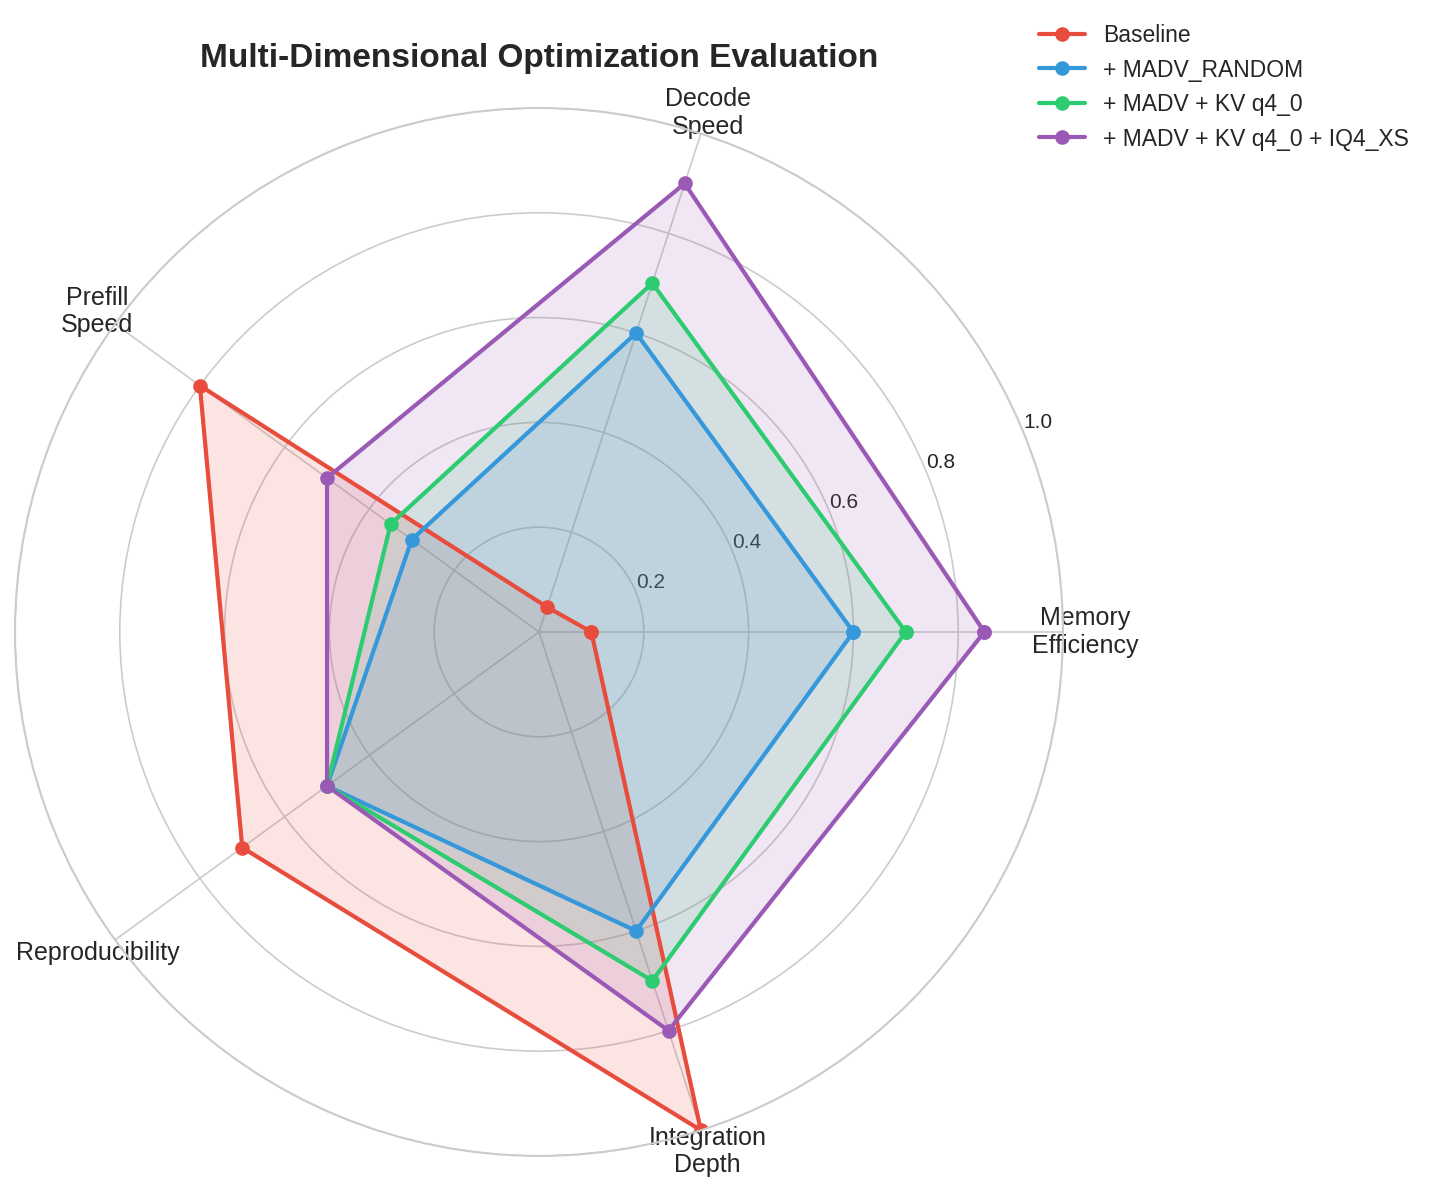
\includegraphics[width=0.65\textwidth]{figures/fig_radar_multimetric.png}
    \caption{多维度优化效果评估雷达图}
    \label{fig:radar}
\end{figure}

\begin{figure}[H]
    \centering
    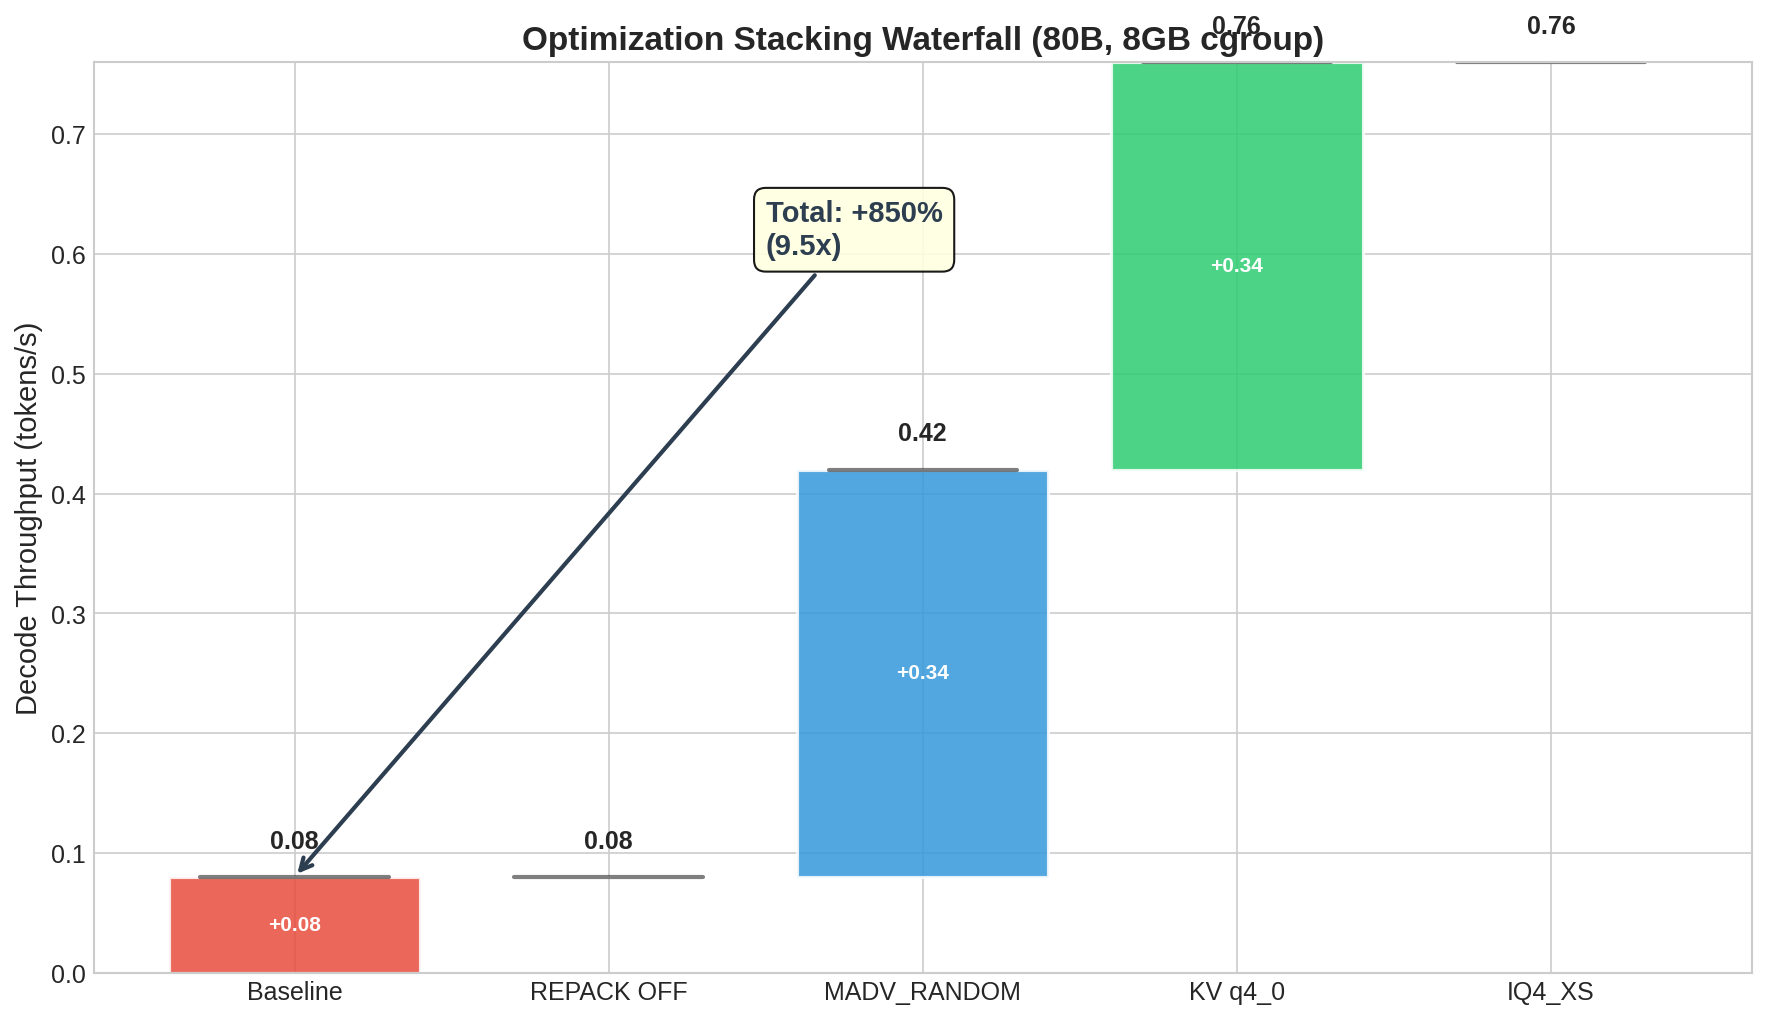
\includegraphics[width=0.9\textwidth]{figures/fig_optimization_waterfall.png}
    \caption{优化技术堆叠瀑布图（80B 8\,GB cgroup）}
    \label{fig:waterfall}
\end{figure}

\begin{figure}[H]
    \centering
    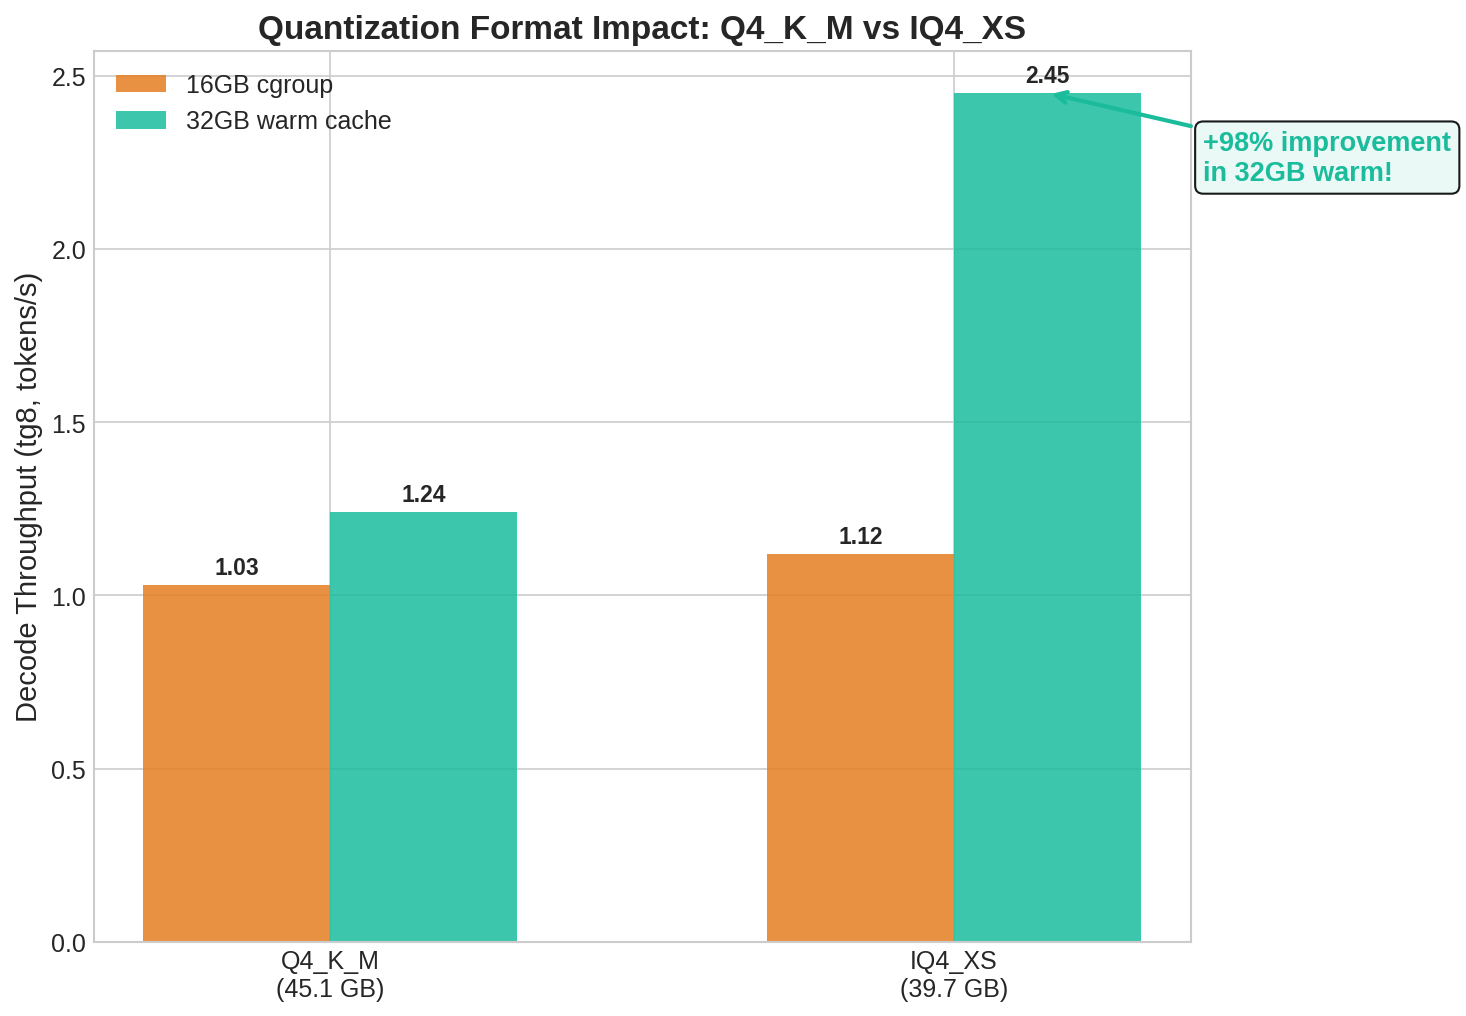
\includegraphics[width=0.85\textwidth]{figures/fig_quant_comparison.png}
    \caption{Q4\_K\_M vs IQ4\_XS 量化格式性能对比}
    \label{fig:quant_compare}
\end{figure}

% Figure: 未来工作路线图
% Prompt: "A roadmap diagram showing current achievements and future work:
%   Current: MADV_RANDOM (done), Repack OFF (done), KV q4_0 (done), IQ4_XS (done)
%   Short-term: Q2_K quantization, KV eviction integration, Prefetch re-evaluation
%   Mid-term: Dynamic MADV switching, Speculative decoding, Tile pipeline
%   Long-term: Unified scheduler validation, Multi-model support
%   Timeline arrows connecting phases. Clean technical style."
